\section{Gestikker}
\label{TestresultaterSocialAcceptGestikker}
%
Følgende analyse og diskusion foretages på baggrund af værternes respons til spørgsmålene: \textit{Hvordan syntes du det var at lære gestikkerne?}, \textit{Havde du problemer med at huske gestikkerne?}, \textit{Hvor rigtigt syntes du, at du fik gengivet gestikkerne til de enkelte funktioner?} og \textit{Var der nogle gestikker, som du følte dig mere ukomfortabel ved at udføre end andre?} samt gæsternes respons til spørgsmålene: \textit{Bemærkede du at din ven(inde)/kæreste lavede gestikker?}, \textit{Kan du gengive de gestikker som din ven(inde)/kæreste lavede?} og \textit{Hvad synes du om dem?}. Derudover inddrages observationer af, hvordan værten reagerer på diverse hints. Første del vil omhandle dels, hvordan værterne vurderer det at lære gestikkerne, om de havde problemer med at huske gestikkerne samt hvor rigtigt de syntes de gengav gestikkerne og dels om gæsterne bemærkede det og var i stand til at gengive dem, samt deres vurdering af gestikkerne. Derefter vil fokus rettes mod om værterne fandt nogle af gestikkerne mere ukomfortable at udføre end andre.\blankline
%
I forhold til hvordan værterne responderede på spørgsmålet: \textit{Hvordan syntes du det var at lære gestikkerne?}, så er den gennemgående tendens, at det var nemt. Vært 2, vært 3 og vært 6 giver alle udtryk for, at gestikkerne kan associeres med hvordan der normaltvist interageres på en telefon, i forhold til swipe-bevægelsen, samt hvordan der normaltvist interageres med et musikanlæg. I det henseende pointerer vært 3 og vært 4, at det er de rigtige gestikker, der er blevet udvalgt til hver funktion og ifølge vært 3 er det nærmest ikke muligt at vælge nogle gestikker, som vil passe bedre. Vært 5 påpeger, at det var en fordel at gestikkerne blev præsenteret via video og ikke på papirform, da det gjorde gestikkerne mere levende. Generelt er der ingen af de seks værter, som giver udtryk for at have problemer med at huske de udvalgte gestikker. Dog kommenterer vært 1, at værten normalvist ikke pauser musikken, når telefonen ringer og derfor var værten, ifølge værten selv, nødsaget til at minde sig selv om det når telefonen ringede. Vært 3 gav udtryk for, at være mere opmærksom på forvrængningen, fordi det er blevet pointeret, af andre, at værten har problemer med hørelsen. Første gang vært 5 skiftede til det næste musiknummer, blev det gjort med hele hånden og eftersom det gik op for værten at det var forkert, så blev det rettet. Det skal dog påpeges at fejlen opstod under familiariseringen, hvorefter værten fejlfrit gengav den korrekte gestik for at skifte til det næste musiknummer. Vært 2 påpeger at fordi gestikkerne ligger i håndleddet, så er der ingen problemer med at huske dem. 

Til spørgsmålet: \textit{Hvor rigtigt syntes du, at du fik gengivet gestikkerne til de enkelte funktioner?} giver de seks værter udtryk for, at de syntes at gestikkerne blev gengivet korrekt. Vært 3 påpeger, at værten kom til at bruge venstre hånd istedet for højre, hvilket ud fra optagelserne skyldes, at værten spiser cookies med højre hånd. Derudover kommenterer vært 3, at værten glemte at starte musikken igen efter den sidste opringning i familiariseringsrunden, fordi værten troede at familiariseringen var færdig, grundet en længere samtale med testleder 2. Vært 4 pointerer, at værten ikke tænkte over det, da der blev reageret på gestikkerne hver gang, så der opstod ikke situationer hvor værten var nødsaget til at repetere gestikkerne. \blankline
%
De seks gæster har alle bemærket, at værten lavede gestikker, men det er ikke alle, der er formår at gengive gestikkerne korrekt, hvilket er illustreret på \autoref{fig:GengiverGestikker}]. Gæst 1 gengiver gestikken til at skrue op og ned korrekt, men er i tvivl om hvilken vej hånden skal dreje for enten at skrue op eller ned. I tillæg bemærker gæst 1, at vært 1 laver en swipe-bevægelse for at skifte musiknummer, men formår ikke at gengive gestikken korrekt. Til gengæld bemærker gæsten ikke, hvilken gestik værten gengiver for at pause eller starte musikken. Gæst 2 kan gengive de forskellige gestikker, dog lukker gæsten hånden i en knytnæve for at pause musikken og swiper med hele hånden istedet for med to fingre. Gæst 3 kan ligeledes gengive gestikkerne korrekt med forbehold for, at gæsten skifter mellem to fingre og hele hånden i swipe-bevægelsen, hvorimod gæst 4 formår at gengive gestikkerne korrekt og uden nogen forbehold. Gæst 5 kan gengive, hvordan musikken pauses, men ikke hvordan den startes igen, hvilket formentlig skyldes, at gæsten slet ikke kigger på værten når musikken startes igen. Derudover formår gæst 5 at gengive gestikken til at skrue op og ned for musikken korrekt og ligesom tilfældet ved de tidligere gæster, gengiver gæst 5 swipe-bevægelsen med hele hånden. Gæst 6 gengiver gestikkerne korrekt, men formår kun at gengive gestikkerne til at pause musikken, skrue ned for musikken og til at skifte musiknummer. 
%
\begin{figure}[H]
	\centering
	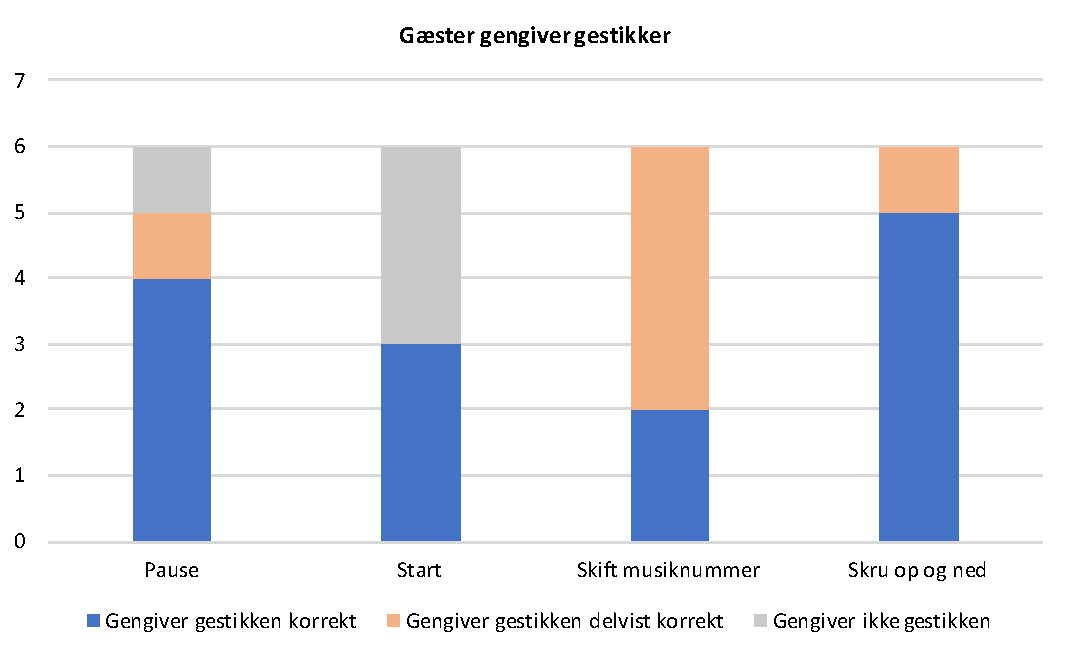
\includegraphics[resolution=300,width=0.9\textwidth]{Test2/GengiverGestikker}
	\caption{Søjlediagram over antallet af gæster, der kan gengive værternes gestikker.}
	\label{fig:GengiverGestikker}
\end{figure}
\noindent
% 
Af resultaterne kan det fastlægges, at gæsterne enten ikke så en specifik gestik, hvilket indikerer at gestikkerne er naturlige og diskrete eller at de så gestikkerne og kan gengive dem rigtigt eller delvist rigtigt, hvilket kan indikere at gestikkerne er nemme at lære. Med delvist rigtigt relateres der til at gæsterne eksempelvis er i stand til at gengive swipe-bevægelsen men ikke nødvendigvis gør det med de to fingre, som gestikken foreskriver eller at de lukker hånden helt i frem for at gengive et krokodillenæb, som gestikken til at pause musikken foreskriver. Ifølge gæst 2 og gæst 5 gav gestikkerne god meningen i forhold til hvilken funktion de tilhører. Gæst 1 tænkte ikke over dem, men giver udtryk for at de var diskrete og fungerede. Derudover kommenterer gæst 1 at værten ikke skulle stå og fægte for at styre musikken. Ifølge gæst 3 er gestikkerne intuitive og derudover kiggede gæsten kun enkelt gang på gestikkerne og vurderede, at de gav god mening og at de var lige til. Gæst 5 pointerer at gestikkerne var nemme og at gæsten selv var i stand til at bruge dem. Den eneste gæst, der udviser en negativ holdning er gæst 6, som giver udtryk for gestikkerne til at starte med er blæret, hvorefter gæsten vil blive træt af dem. Gæsten giver udtryk for at det er et fedt festtrick men forestiller sig, at det er træls når der er flere mennesker.
%
\subsection{Var der nogle gestikker, som du følte dig mere ukomfortabel ved at udføre end andre?}
\label{TestresultaterSocialAcceptGestikkerUkomfortabelt}
%
Ud af de seks værter er det kun vært 1 og vært 6, som direkte giver udtryk for, at en af gestikkerne føltes mere ukomfortabel end de andre; den til at skrue op og ned for musikken. Tre af de fire værter, som ikke oplevede at nogen gestikker var mere ukomfortable at udføre end andre, giver udtryk for bekymringer relateret til den specifikke gestik. Vært 5 kommenterer, at der derudover kan være noget kulturelt ved gestikken til at pause musikken, som kan misforståes, i og med at det forbindes med en "klap i"-bevægelse. Dog pointere vært 5 at ingen i værtens omgangskreds vil misforstå gestikken, hvorfor det ikke vil opstå et problem. Vært 3 og vært 4 giver begge udtryk for bekymringer relateret til gestikken, som er tilknyttet skru op og ned. Fælles for de to værter er, at de giver udtryk for, at der kan opstå problemer i forhold til hvor meget der skal drejes for at skrue en hvis mængde op eller ned. Hvor vært 3 ydermere kommenterer, at gestikker kræver mere finmotorik sammenlignet med de andre udvalgte gestikker. Derudover påpeger værten, at det kan være et problem, hvis bevægelsen kræver en helt rolig og præcis hånd for at kontrollere volumen. I tillæg kommenterer værten at ved fysisk kontakt, eksempelvis med en drejeknap, så er det muligt at lave en mindre bevægelse sammenlignet med semaforiske gestikker, fordi den fysiske kontakt tillader bedre føling med den pågældende knap. 

Der er to årsager til at vært 1 finder gestikken til at skrue op og ned for musikken mere ukomfortabel end de andre gestikker; 1) der er risiko for, at der pludseligt skrues for højt op og 2) hvis rotationen begyndes et dårligt sted, så håndleddet fysisk ikke tillader mere rotation. Værten påpeger dog, at hvis grænsen for, hvor meget ens håndled kan roteres nåes, så kan grebet slippes, hvorefter det er muligt at gribe fat igen. Grebet referer til, at der tages fat i en imaginær drejeknap. Vært 6 giver udtryk for, at der var noget underligt med responsen, når værten skruede op og ned. Dette kan formentlig skyldes flere ting; dels at det er testleder 2, som styrer volumen afhængigt af værtens gestikulering, så i tilfælde af at det ikke blev gjort i overensstemmelse med værtens forventning, så er det forståeligt, at responsen kan virke underlig. Derudover kan det skyldes, at testleder 2 havde svært ved præcis at tolke bevægelsesmængden i vært 6's gestikulering, da fingrenes position ændrede sig i takt med rotationen. Derudover påpeger vært 6, at det kræver tilvænning i forhold til hvor meget der skal drejes og hvornår rotationen skal stoppe. Dog pointerer værten, at volumen normaltvist ikke ændres fra 0 til 100. 
%
\section{Observationer af vært og gæst}
\label{TestresultaterSocialAcceptGestikkerObservationer}
%
I følgende afsnit analyseres og diskuteres observationer fra videooptagelserne af de seks par. Observationerne dækker blandt andet over om gæsterne spørger ind til gestikkerne, hvordan værternes interaktion med musikanlægget forløber og hvordan samtalen mellem vært og gæst påvirkes af værtens interaktion med musikanlægget.
%
\subsection{Spørger gæsterne ind til gestikkerne}
\label{TestresultaterSocialAcceptGaestSPGGestikker}
%
Baseret på videooptagelserne er der ingen af gæsterne, der decideret spørger ind til værtens gestikker. Gæst 3 kommenterer når værten bliver bedt om at indstille volumen til et passende samtale niveau ved det første musiknummer. Kommentaren retter sig ikke direkte mod selve gestikken men mod det, at værten bruger gestikker, hvor gæsten giver udtryk for, at det er fedt. I musiknummer 2 reagerer gæst 3 på, at musikken bliver skruet højt op og forsøger selv at skrue ned. Dette gøres dog i takt med at værten selv skruer ned, hvorfor det er værtens gestik testleder 2 reagerer på. Gæst 3 giver udtryk for gerne, at ville prøve gestikkerne, men det realiseres ikke, da samtalen drejes tilbage på ferieplanlægningen. Gæst 4 kommenterer ligeledes, når værten i starten skal indstille volumen til et passende samtale niveau. Igen rettes kommentaren ikke direkte mod selve gestikken, men mod det, at der bruges gestikker, hvorefter gæsten selv får lov til at prøve at indstille volumen og spørger efterfølgende ikke ind til gestikkerne igen. De fire resterende gæster hverken prøver eller kommenterer på værtens gestikker. At gæsterne ikke direkte spørger ind til gestikker skyldes formentligt at det er en testsituation og at gæsterne informeres om, at værten har fået et musikanlæg, som de hører musik fra og at værten i den forbindelse skal interagere med anlægget. Det antages at gæsterne i en virkelig situation formentlig vil være nysgerrige og spørge ind til interaktionsformen. Med udgangspunkt i det foregående samt gæsternes respons i exit-interviewet, så tyder det ikke på at denne interaktionsform tiltrækker negativ opmærksomhed. 
%
\subsection{Hvordan værtens interaktion med musikanlægget forløber}
\label{TestresultaterSocialAcceptVaertsGestikker}
%
I følgende afsnit fokuseres der på; hvordan værterne generelt gestikulerer, når de ikke reagerer på hints, om værterne begår fejl, og hvis de gør, hvornår og hvilke fejl begåes. Derudover fokuseres der på om værterne interagerer med musikken uden der har været et hint, om nogen af værterne bruger venstre hånd frem for højre, hvor mange gange værterne retter fokus mod enten anlægget, kommunikationskameraet eller selve gestikken og hvor mange gange gæsterne retter fokus mod værternes gestikker eller hints.\blankline
%
I forhold til hvordan værterne generelt gestikulerer, når de ikke reagerer på hints, så er værterne generelt meget stillesiddende og ingen af værterne laver gestikker, som misforståes af testleder 2. Dog laver vært 4 en "pyt-med-det"-bevægelse, som tilnærmelsesvist minder om et swipe med hele hånden, bortset fra at værtens bevægelsen er mere vertikal end horisontal. Værtens "pyt-med-det"-bevægelse kommer kun én gang og kommer i forbindelse med at værten og gæsten taler om budgetterne til de tre ferier. Ud fra observationerne af vært 2, så tyder det på, at værten koncentrerer sig om at høre de forskellige hints, eksempelvis retter værten ofte fokus mod mobiltelefonen, selvom den ikke ringer.\blankline
%
Fokuseres der på, om værterne begår fejl under udførelsen af gestikkerne, er det vært 1, vært 3, vært 4 og vært 5 der laver direkte fejl i gestikken. Ved vært 4 og 5 drejer det sig om to enkeltstående tilfælde, hvor værterne skifter sang ved at lave en swipe bevægelse med én finger i stedet for to. Hvor vært 1 ved den sidste opringning glemme at pause musikken og dermed heller ikke formår at starte musikken igen. Som tidligere nævnt kommenterer vært 1, at værten normalvist ikke pauser sin musik ved et opkald. Vært 3 skifter, i musiknummer 4, musiknummer med hele hånden fremfor de to fingre gestikken foreskriver. Generelt skifter vært 3 musiknummer med en lidt doven hånd, der ofte starter swipe-bevægelsen med to fingre og ender med hele hånden. For at undersøge om vært 3 under familiariseringen har lært at gengive den korrekte gestik til at skifte musiknummer, foretages der observationer af værtens familiarisering. Baseret på disse observationer vurderes det, at værten rent faktisk har lært at gengive den korrekte gestik og gengiver den korrekt under hele familiariseringen, dog swiper værten, som nævnt, med en doven hånd. Der er derfor ikke mistanke om at værten har misforstået hvordan gestikken skal udføres, men derimod tyder det på at værten udfører gestikken mere dovent desto mere fortrolig værten bliver med gestikken. Derudover bygger observationerne på optagelserne foretaget med GoPro-kameraet, som er placeret modsat kommunikationskameraet, hvilket potentielt kan have indflydelse på hvordan værtens gestikker vurderes. Baseret på testledernes observationer inde fra kontrolrummet er værten kun noteret for en enkelt fejl, hvor værten swipede med hele hånden, det tyder derfor på at GoPro-kameraets vinkel har gjort det svært at genkende gestikken efterfølgende. 

Da vært 1, vært 4 og vært 5 hver især kun begår en enkelt fejl vurderes det, at det ikke er nødvendigt at undersøge deres familiarisering nærmere.\blankline
%
Når værterne interagerede med musikanlægget uden hints, blev det ikke noteret som en fejl, da brugere i en virkelig situation selvfølgelig skal kunne interagere med sit musikanlæg på ethvert tidspunkt. Interaktionerne uden hints relaterer sig nærmest udelukkende til at skrue op og ned for musikken i forbindelse med, at værten tidligere har skruet for meget ned eller for højt op. 

Ydermere skifter vært 1, vært 2 og vært 6 musiknummer, uden at der har været et hint, hvilket påvirker præsentationen af de efterfølgende hints og resulterer i at værterne ikke præsenteres for lige mange hints. Vært 1 skiftede musiknummer i slutningen af det musiknummer, som afspilles først for at få samtalen ordentlig i gang før de planlagte hints efterfølgende præsenteres. Årsagen til at værten skiftede musiknummer begrundes med at værten syntes at outtroen var irriterende og da dette ikke har en betydningen for rækkefølgende hvorved de forskellige hints præsenteres grab testlederne ikke ind. I den første opringningen fik værten dog at vide, at der fremover kun skal reageres på hints, hvilket værten, med undtagelse af en justering af volumen, overholdte. Ligesom tilfældet med vært 1 så skifter vært 2 ligeledes musiknummer i det første musiknummer, men denne gang sker det tidligt i musiknummeret, hvilket resulterer i at testleder 2 ringer til værten og spørger ind til om højttalerne skratter og derudover beder værten om kun at reagere på hints. Efter opkaldet startes musiknummeret forfra, og vært og gæst forstætter ferieplanlægningen. Efterfølgende skifter vært 2 ikke musiknummer uden et hint.    

Ved musiknummer 1 skifter vært 6 til det næste musiknummer, uden at der har været et hint, hvilket testleder 2 reagerer på, da det næste hint alligevel vil være forvrængningen, som netop skal få værterne til at skifte musiknummer og da vært 6 skifter musiknummer få sekunder før hintet, vurderes det til ikke at være en fejl. I musiknummer 4 vil vært 6 igen skifte musiknummer og da dette sker samtidig med at testleder 2 er i gang med at ringe op til værten, så reageres der ikke på at værten vil skifte musiknummer. Under opringningen får værten at vide, at der kun skal reageres på hints, hvor vært 6 begrunder sin interaktion med, at musikken var af dårlig kvalitet. Efterfølgende reagerer vært 6 kun på de resterende hints.\blankline
%
Som forklaret er det kun højrehåndede testpersoner, der vælges til at agere værter, hvorfor det forventes at gestikkerne kun udføres med højre hånd. Baseret på observationerne er der dog to værter; vært 3 og vært 6, som benytter sig af venstre hånd til at interagere med musikken, hvilket skyldes at begge værter spiser cookie med højre hånd. Det er bemærkelsesværdigt at vært 3 swiper fra venstre mod højre, når værten gestikulerer med venstre hånd, hvorimod vært 6 swiper fra højre mod venstre med venstre hånd. Da der kun er opsat krav til hvordan interaktionen ved swipe skal foregå med højre hånd, er det ikke muligt at konkludere om værterne gør det korrekt med venstre hånd. Dette lægger op til en undersøgelse af hvordan interaktionen reelt skal foregå med venstre hånd når brugeren enten er højrehåndede eller venstrehåndede, da der uundgåeligt vil være venstrehåndede brugere i Bang $\&$ Olufsens kundekreds.     
%
\begin{figure}[H]
	\centering
	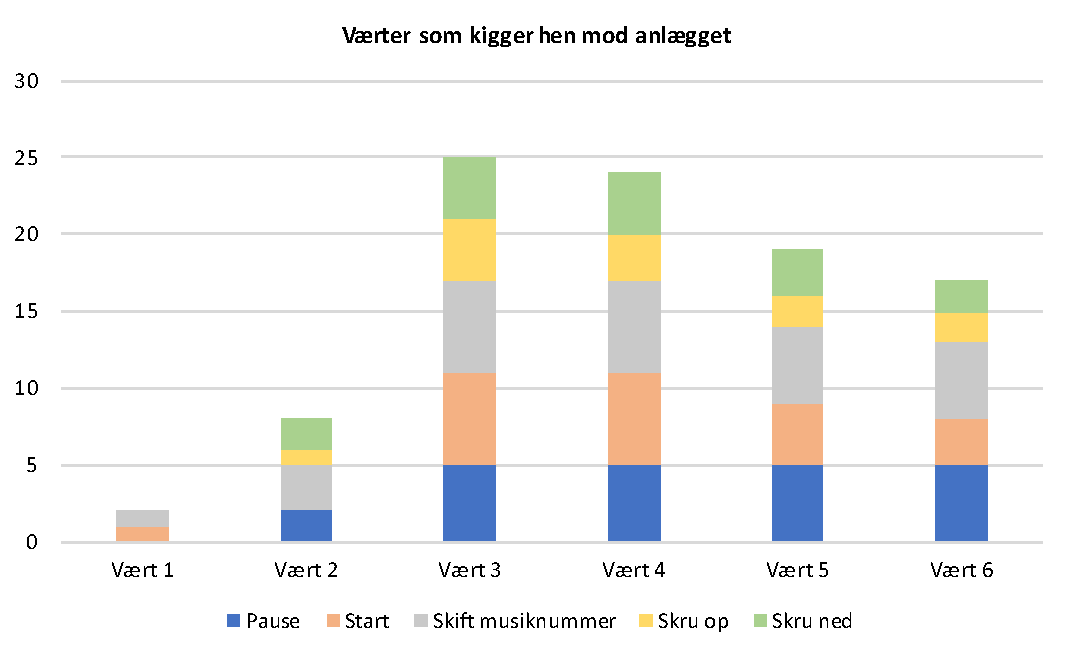
\includegraphics[resolution=300,width=0.9\textwidth]{Test2/KiggerImodAnlaeg}
	\caption{Søjlediagram over antallet af gange værterne kigger hen mod anlægget ved hver funktion. Data bygger på observationerne fra videooptagelserne af vært og gæst.}
	\label{fig:KiggerImodAnlaeg}
\end{figure}
\noindent
% 
Når værterne interagerer med musikanlægget, er det forskelligt hvem og hvor mange gange værternes blik rettes i den retning, jævnfør \autoref{fig:KiggerImodAnlaeg}. Vært 1 interagerer oftest med musikanlægget uden at kigge i den retning, modsat vært 3 og vært 4, som stort set kigger mod musikanlægget, hver gang de interagerer med det. Afhængigt af hvordan værten interagerer med musikanlægget er det derfor interessant, at undersøge dels om det påvirker samtalen og dels om det påvirker gæstens indtryk af interaktionsformen. For at undersøge dette nærmere sammenholdes observationerne af hvordan værterne interagerer med musikanlægget samt hvor mange gange de kigger i den retning med om de respektive gæster er i stand til at gengive værtens gestikker. 

Gæst 1 reagerer kun to gange på, at værten interagerer med musikanlægget, hvilket særligt kommer til udtryk, da gæsten kun delvist kan gengive gestikkerne til henholdvis at justere lydstyrken og til at skifte musiknummer, men slet ikke kan gengive pause og start. Ved par 2 fremgår det tydeligt ud fra observationerne, at så snart værten får at vide, at gestikkerne gerne må laves mere diskret, så kigger værten færre gange mod musikanlægget, hvilket mindsker gæstens reaktion på interaktionen. Som tidligere nævnt kan gæst 2 gengive samtlige gestikker korrekt eller delvist korrekt, hvilket højst sandsynligt skyldes at gæsten reagerede brat på værtens tydelige interaktion med musikanlægget i starten af testen. 

For par 3 og par 4 er situationen ens; selvom værterne kiggede hen mod musikanlægget næsten hver gang de interagerede med det, så var gæsterne primært fascinerede af interaktionsformen i starten, hvorefter fokus blev rettet mod ferieplanlægningen. Begge gæster kommenterede på gestikkerne og gæst 4 prøvede selv at justere lydstyrken, hvilket kan have indflydelse på den dalende interesse. Jævnfør \autoref{fig:KiggerImodAnlaeg} kigger vært 5 ofte hen imod musikanlægget ved interaktion, og ud fra observationerne af optagelsen af par 5 fremgår det, at værten oftere kigger hen imod anlægget i slutningen af testen end i starten, årsagen er dog uvis. Selvom værten ofte vender blikket mod anlægget, så lader det ikke til at påvirke gæsten, da gæsten ikke på noget tidspunkt virker til at interessere sig for eller reagere på gestikkerne. Gæsten retter derimod sin opmærksomhed mod værtens ansigt eller ferieplanlægningen. 

At disse tre gæster; gæst 3, gæst 4 og gæst 5 bliver mindre påvirket af interaktionen, selvom den respektive vært ofte vender blikket mod anlægget og eller gestikken, kan skyldes at værterne gestikulerer diskret og samtidig interagerer naturligt med musikanlægget.

Ligesom ved vært 2, så kigger vært 6 ofte hen i mod musikanlægget og gestikulerer tydeligt på hints, indtil værten i et opkald får at vide, at gestikkerne gerne må laves mere diskrete, hvorefter værten ikke kigger lige så ofte mod anlægget som før. Inden værten får opkaldet fremgår det tydeligt at gæst 6 ligeledes reagerer brat på interaktionen og at det forstyrrer deres samtale, så snart værten laver gestikkerne diskret, så reagerer gæsten stort set ikke på værtens resterende gestikker. Det antages, at såfremt vært 6 tidligere i testen havde fået besked på at gøre gestikkerne mere diskrete, så ville værten ikke kigge hen imod anlægget lige så mange gange, som det er tilfældet, jævnfør \autoref{fig:KiggerImodAnlaeg}. 

Der vil i følgende afsnit fokuseres yderligere på hvordan samtalen mellem vært og gæst påvirkes af værtens interaktion med musikanlægget.
%
\subsection{Hvordan påvirkes samtalen mellem vært og gæst}
\label{TestresultaterSocialAcceptSamtale}
%
I følgende afsnit fokuseres der på; hvordan samtalen mellem vært og gæst påvirkes af værtens interaktion med musikanlægget og om værten selv benytter sig af computeren eller papirerne, som gæsten har medbragt. \blankline
%
Baseret på observationerne af de seks par, tyder det på, at det primært er ved par 2 og par 6, at samtalen påvirkes mellem vært og gæst. Ved par 2 tyder det på, at samtalen afbrydes, fordi værten koncentrerer sig om at registrerer og reagerer på hints, hvilket får gæsten til at stoppe op og vente til værten er færdig. Dette ændres dog efter værten får at vide dels, at værten gerne må benytte sig af computeren, hvilket sker i opringningen i musiknummer 1 og dels når værten bliver opfordret til at gøre gestikkerne mere diskrete, hvilket sker i opringningen i musiknummer 2. Efterfølgende tyder det på at samtalen mellem vært og gæst ikke påvirkes i lige så høj grad som før og at værten ikke koncentrerer sig lige så meget om at registrere diverse hints. Ud fra både observationer og værtens egen respons i exit-interviewet, så tyder det på, at værten havde problemer med at registre forvrængningen. I forhold til par 6, så tyder det på, ud fra observationerne, at hver gang værten reagerer på et hint, så tiltrækker det gæstens opmærksomhed, hvilket afbryder samtalen, dog er de begge i stand til at vende hurtigt tilbage til samtaleemnet. Årsagen til at værtens interaktion med musikanlægget tiltrækker gæstens opmærksomhed er formentlig fordi at værten både retter sit fokus og sin krop mod anlægget, som er placeret modsat gæsten, hvilket derfor resulterer i, at gæsten ligeledes retter fokus fra samtalen til værtens interaktion. I opringningen i musiknummer 4 opfordres vært 6, som nævnt, til at lave gestikkerne mere diskrete, hvorefter det tyder på, at samtalen ikke længere påvirkes i lige så høj grad. Det tyder på, at både opringningen og det, at værten for alvor begynder at bruge gæstens medbragte computer er med til dels, at samtalen ikke afbrydes lige så brat som før og dels, at værten interagerer med musikanlægget mere afslappet og uden både at rette sit fokus og sin kroppen mod anlægget.

Ud fra observationerne af de resternede fire par; par 1, par 3, par 4 og par 5, så tyder det ikke på at værtens interaktion med musikanlægget har påvirket samtalen med gæsten negativt. Når vært 1 reagerer på en opringning arbejder gæsten som regel videre med ferieplanlægningen, hvorefter værten hurtigt falder ind i samtalen igen. Baseret på observationerne af par 3 tyder det på, at den eneste gang et hint påvirker samtalen er ved musiknummer 4, hvor der bliver skruet højt op for musikken, hvilket får gæsten til at reagerer. Generelt tyder det ikke på, at samtalen mellem vært 3 og gæst 3 påvirkes negativt, da de holder sig til samtaleemnet og samtidig inkluderer opkaldende som en naturlig del af deres samtale. Lignende er gældende for par 5, hvis samtale ikke påvirkes af diverse hints og hvor værten ligeledes inkluderer opkaldende som en naturlig del af deres samtale. Ud fra observationerne af par 4 tyder det heller ikke på, at værtens interaktion med musikanlægget påvirker samtalen med gæsten negativt, da både vært og gæst formår at opretholde samtalen og gæsten arbejder videre, når værten reagerer på et opkald. \blankline
%
I forhold til om værterne benytter sig af gæstens medbragte computer eller de medbragte papirer, så benytter halvdelen af værterne sig af computeren og ingen benytter papirene. Vært 2 benytter sig af computeren allerede efter den første opringning i musiknummer 1 og benytter den stort set resten af tiden. Vært 5 benytter computeren i starten af musiknummer 3, hvor gæsten hurtigt overtager inden værten reagerer på hintet om at skifte musiknummer og kortvarigt i musiknummer 6. Vært 6 benytter computeren kortvarigt i musiknummer 1 og igen efter opkaldet i musiknummer 4, hvorefter værten benytter sig af computeren stort set resten af tiden. 

På baggrund af observationerne vurderes det, med forbehold for at vært 2 og vært 6 først skulle opfordres til at gestikulere mere diskret, at værternes interaktion med musikanlægget ikke påvirkede samtalen med gæsten negativt. Ydermere opstod der ikke akavede pauser mellem vært og gæst hvor de ikke vidste, hvad de skulle sige til hinanden eller hvor de kom fra. 

